\section{Evaluation}
\label{sec:evaluation}

This section has two goals. First, we want to compare our fragmentation approach to other model persistence frameworks. Secondly, we want to verify our findings from section~\ref{sec:gains}. 
All measurements were performed on a Computer with Intel Core i5 2.4\.GHz CPU, 8 GB 1067 MHz DDR3 RAM, running Mac OS 10.7.3. All experiments were repeated at least 20 times, and all present results are respective averages. Code executing all measurements and all measured data can be downloaded as part of EMFFrag~\cite{EMFFragProject}.

\subsection{Fragmentation Compared to other Persistence Frameworks}

To compare fragmentation to EMF XMI, CDO, and Morsa, we measured execution time for the abstract modeling task. To analyse traverse and query, we used example models from the Grabats 2009 contest~\cite{grabats} as benchmarks. Those were already used to compare Morsa with EMF XMI and CDO here~\cite{morsa2011}. There are five example models labelled \emph{set0} to \emph{set4} and they all model Java software based on the same meta-model. Please note: even though the models increase in size, their growths is not linear. To measure the last task create/modify, we use simple test models, because importing Grabats' large XMI models files does not allow effective separation of loading the models with EMF and storing them with the respective persistence framework. We don't provide any comparative measures for partial loads. Partial load performance is indirectly covered by the measures on queries, which required to partially load the Grabats models. Furthermore, partial loads are extensively measured for EMFFrag in the next section.

Fig.~\ref{fig:grabatsFragments} shows the number of fragments that each framework produces for each model. Morsa and CDO implement total fragmentation and the number of fragments is also the number of objects in the model. For EMF XMI there is always only one fragment, because it implements no fragmentation. For EMFFrag, we provided two different meta-model based fragmentations. The first one puts each Java compilation unit and class file into a different fragment (EMFFrag coarse). The second one additionally puts the ASTs for each method block into a different fragment (EMFFrag fine). The number of fragments differs significantly for \emph{set2} and \emph{set3} which obviously contain a lot of method definitions. 

We could not measure CDO's performance for \emph{set3} and \emph{set4}: the models are to large for a single CDO transaction, and circular cross-references do not allow to import the model with different transactions.

\begin{figure}[ht]
\begin{minipage}[b]{0.48\linewidth}
\centering
\includegraphics[width=\linewidth]{figures/grabatsTraverseTimeExtra}
\caption{Execution time for traversing the different Grabats models with the different persistence solutions.}
\label{fig:grabatsTraverseTime}
\end{minipage}
\hspace{0.02\linewidth}
\begin{minipage}[b]{0.48\linewidth}
\centering
\includegraphics[width=\linewidth]{figures/grabatsQueryTimeExtra}
\caption{Execution time for querying the different Grabats models with the example query.}
\label{fig:grabatsQueryTime}
\end{minipage}
%\end{figure}
%\begin{figure}[ht]
\begin{minipage}[b]{0.48\linewidth}
\centering
\vspace{0.04\linewidth}
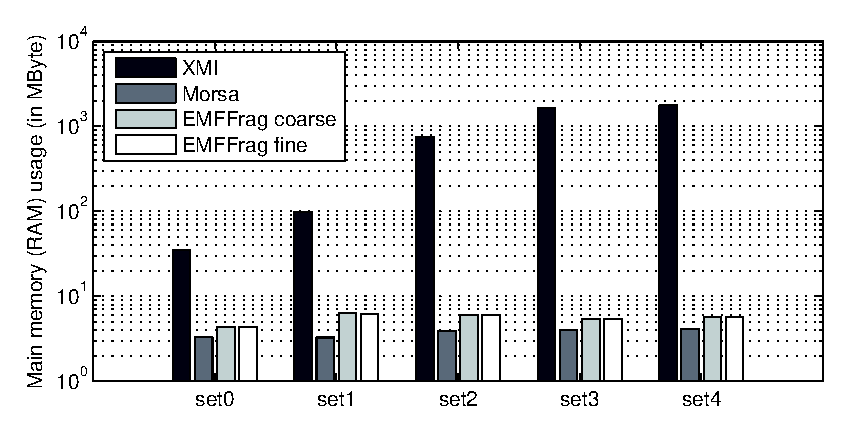
\includegraphics[width=\linewidth]{figures/grabatsTraverseMem}
\caption{Memory usage time for traversing the different Grabats.}
\label{fig:grabatsTraverseMem}
\end{minipage}
\hspace{0.02\linewidth}
\begin{minipage}[b]{0.48\linewidth}
\centering
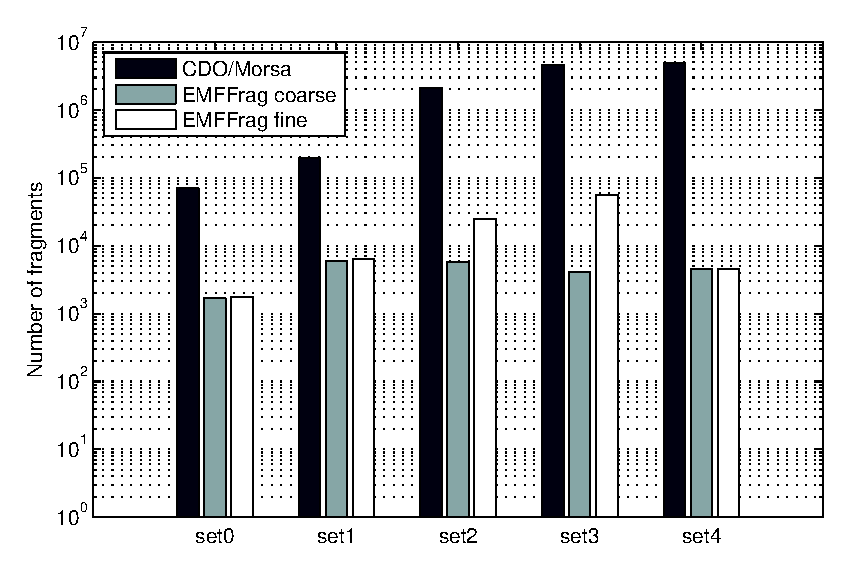
\includegraphics[width=\linewidth]{figures/grabatsFragments}
\caption{Number of fragments used by the different persistence solutions.}
\label{fig:grabatsFragments}
\end{minipage}
\end{figure}

\subsubsection*{Create/Modify} \markus{Big TODO: I need to measure this, describe the test models, plot results and testmeta-model and describe the results.}

\markus{Lorem ipsum dolor sit amet, consetetur sadipscing elitr, sed diam nonumy eirmod tempor invidunt ut labore et dolore magna aliquyam erat, sed diam voluptua. At vero eos et accusam et justo duo dolores et ea rebum. Stet clita kasd gubergren, no sea takimata sanctus est Lorem ipsum dolor sit amet. Lorem ipsum dolor sit amet, consetetur sadipscing elitr, sed diam nonumy eirmod tempor invidunt ut labore et dolore magna aliquyam erat, sed diam voluptua. At vero eos et accusam et justo duo dolores et ea rebum. Stet clita kasd gubergren, no sea takimata sanctus est Lorem ipsum dolor sit amet.}

\markus{Lorem ipsum dolor sit amet, consetetur sadipscing elitr, sed diam nonumy eirmod tempor invidunt ut labore et dolore magna aliquyam erat, sed diam voluptua. At vero eos et accusam et justo duo dolores et ea rebum. Stet clita kasd gubergren, no sea takimata sanctus est Lorem ipsum dolor sit amet. Lorem ipsum dolor sit amet, consetetur sadipscing elitr, sed diam nonumy eirmod tempor invidunt ut labore et dolore magna aliquyam erat, sed diam voluptua. At vero eos et accusam et justo duo dolores et ea rebum. Stet clita kasd gubergren, no sea takimata sanctus est Lorem ipsum dolor sit amet.}

\subsubsection*{Traverse} The execution times of CDO, Morsa, and EMFFrag are proportional to the size of the model (Fig.~\ref{fig:grabatsTraverseTime}). Times for EMF XMI grow faster than the model's sizes. Interestingly, Morsa and CDO both use total fragmentation and their respective execution times are very close. EMFFrag performs significantly faster: upto 10 times as fast as Morse and CDO. For models \emph{set2} and \emph{set3} (where the number of fragments differ largely between fine and coarse fragmentation) the fine fragmentation performs (not surprisingly) worse, since more fragments have to be loaded.

\subsubsection*{Query} The Grabats contest also provides an example query: find all Java type declarations that contain a static method which has this declared type as return type. Depending on the persistence framework, queries can be implemented in different ways. With EMF XMI and EMFFrag there are not indexes that would help to implement the query and we have to traverse the model until we found all type declarations. CDO allows to use SQL to query and Morsa provides a meta-model class to objects index. We measured both: executing the queries with these specific query mechanisms and with the previously mentioned traverse based implementation.

The results (Fig.~\ref{fig:grabatsQueryTime}: EMF XMI performs badly for large models. CDO and Morsa with SQL and meta-class index performs best. But even though EMFFrag needs to traverse the model its performance is similar to CDO and Morsa. For \emph{set3} and fine fragmentation, EMFFrag even outperforms Morsa's index. Remember, with the fine fragmentation, EMFFrag does not need to load any method bodies to execute the query (partial load). Using the traverse implementation, CDO's and Morsa's performance difference to EMFFrag is similar to the measures for model traverse (here we basically perform a partial traverse).  

\subsubsection*{Memory usage} During model traverse, we also measured the memory usage (Fig.~\ref{fig:grabatsTraverseMem}). EMF/XMI's memory usage is proportional to model size, because it needs to load the full models into memory. All other approaches need a comparable constant quantity of memory independent of model size.


\subsection{The Influence of Fragmentation on Partial Load Performance}

In section~\ref{sec:gains}, we looked at fragmentation analytically and provided a plot (Fig.~\ref{fig:theoryTimesSmall}) that describes the expected influence of fragmentation granularity on partial load execution times. Here, we create the same plot, but based on data measured with EMFFrag. For this purpose, we used a simple meta-model (ref. to Fig.~\ref{?}) and generated models of size $10^6$ with different fragment sizes $f$. We measured the execution times for loading parts of different sizes $l$. The results are presented in Fig.~\ref{fig:measureTimeExtra}.

\begin{figure}
  \centering
  \includegraphics[width=0.65\linewidth]{figures/measureTimesExtra}
  \caption{Execution times for loading model parts with different fragmentation granularities.}
  \label{fig:measureTimeExtra}
\end{figure}

The plots show a similar picture with comparable values. Although, the measured times are generally larger probably due to additional EMFFrag implementation overhead that was not considered in our theoretical examination.